\section{Технологический раздел}

В данном разделе будут выбраны средства реализации программного обеспечения, описаны основные функции разработанного программного обеспечения, приведены результаты тестирования, примеры пользовательского интерфейса, демонстрация работы программы, а также руководство пользователя.

% NOTE:
% Технологический раздел содержит обоснованный выбор средств программной реализации, описание основных (нетривиальных) моментов разработки и методики тестирования созданного ПО
% В этом же разделе описывается информация, необходимая для сборки и запуска разработанного ПО, форматы входных, выходных и конфигурационных файлов (если они имеются), а также интерфейс пользователя и руководство пользователя
% Часть технологического раздела должна быть посвящена тестированию разработанного ПО
% Модульное тестирование описывается в технологическом разделе
% Системное тестирование может быть описано в технологическом или исследовательском разделах

% Рек. Объем 20-25 страниц

\subsection{Выбор средств реализации}

% Обосновать выбор программных средств реализации предложенного метода

Для реализации метода выделения составных частей научного текста на основе анализа распределения пикселей в сканирующей строке был выбран Python~\cite{python} по следующим причинам:
\begin{itemize}
    \item язык программирования позволяет быстро создавать рабочие прототипы в связи с наличием большого количества библиотек;
    \item имеются библиотеки для работы с PDF документами и изображениями;
    \item есть опыт работы с данным языком программирования.
\end{itemize}

Для управления зависимостями Python-проекта и организации изолированных виртуальных окружений, обеспечивая воспроизводимость и независимость среды выполнения, был выбран uv~\cite{uv}.

Для работы с массивами данных (в том числе сканирующей строкой пикселей) была выбрана библиотека NumPy~\cite{numpy}.

Для работы с изображениями и PDF были выбраны библиотеки PIL~\cite{pil} и PyMuPDF~\cite{pymupdf} соответственно, так как в процессе работы программы используются как PDF документы, так и изображения, а PyMuPDF позволяет преобразовывать результат рендеринга PDF в формат, поддерживаемый PIL, который, в свою очередь, может быть преобразован в NumPy массив и использован для дальнейшей обработки.

Для создания веб-интерфейса была выбрана библиотека Gradio~\cite{gradio}, так как данная библиотека позволяет быстро создать рабочий прототип графического интерфейса к программе.

В качестве среды разработки был выбран Neovim~\cite{nvim} по следующим причинам:
\begin{itemize}
    \item данный текстовый редактор позволяет редактировать файлы с исходным кодом программы;
    \item быстрая и удобная навигация по файлам проекта;
    \item есть опыт использования данного текстового редактора.
\end{itemize}

\subsection{Реализация программного обеспечения}

В данном подразделе будут описаны входные и выходные данные основных функций разработанного программного обеспечения, а также приведены их листинги.

% Описать формат входных и выходных данных

\subsubsection{Точка входа}
Входные данные:
\begin{itemize}
    \item pdf\_path --- строка, путь к PDF документу,
    \item json\_path --- строка, имя создаваемого файла разметки;
    \item markup\_type --- целое число от 0 до 3, тип разметки; 0 --- построчная разметка, 1 --- первичная разметка, 2 --- уточненная разметка, 3 --- объединенная разметка.
    \item num\_workers --- целое число, число рабочих процессов, так как документ быстрее обрабатывать параллельно;
    \item page\_indices --- массив целых чисел, конкретные страницы для обработки, если они указаны; по умолчанию обрабатывается весь документ.
\end{itemize}

Выходные данные: Сохраненная в указанном JSON файле разметка.

Исходный код данной функции приведен в листинге~\ref{lst:mainf} ниже.

\newpage

\begin{lstlisting}[caption={Точка входа, функция main}, label={lst:mainf}]
def main(pdf_path, json_path, markup_type, num_workers=8, page_indices=None):
    results = []

    if page_indices is None:
        doc = fitz.open(pdf_path)
        total_pages = doc.page_count
        page_indices = list(range(total_pages))
        doc.close()

    # Делит диапазон страниц на N примерно равных кусков.
    chunks = chunk_indices(len(page_indices), num_workers)
    pages_chunks = [ [page_indices[i] for i in chunk] for chunk in chunks ]

    # .. (Создание шкалы прогресса и запуск ее в отдельном потоке)

    try:
        with ProcessPoolExecutor(max_workers=num_workers) as executor:
            futures = [executor.submit(process_pages, pdf_path, chunk, markup_type,
                                       queue) for chunk in pages_chunks]
            for future in futures:
                results.extend(future.result())
    finally:
        stop_signal.set()
        thread.join()

    results.sort(key=lambda x: x["page"])

    with open(json_path, "w", encoding="utf-8") as f:
        json.dump(results, f, ensure_ascii=False, indent=4)

    return results
\end{lstlisting}

\subsubsection{Функция обработки страниц}

Данная функция запускается для каждого процесса, после чего результаты обработки страниц объединяются.

Входные данные:
\begin{itemize}
    \item pdf\_path --- строка, путь к PDF документу,
    \item page\_range --- целочисленный массив, страницы, которые требуется обработать конкретному процессу;
    \item markup\_type --- целое число от 0 до 3, тип разметки;
    \item queue --- объект типа очередь, нужен исключительно для обновления строки прогресса в терминале.
\end{itemize}

Выходные данные: Частичная разметка в виде Python-словаря указанного в листинге \ref{lst:pp} формата.

Исходный код данной функции приведен в листинге~\ref{lst:pp} ниже.

\begin{lstlisting}[caption={Функция обработки страниц}, label={lst:pp}]
from fast import segdoc as sd
def process_pages(pdf_path, page_range, markup_type, queue=None):
    """Функция для обработки поддиапазона страниц."""
    partial_results = []
    for i in page_range:
        image = page_to_image(pdf_path, i)
        image_np = np.array(image)
        markup = sd(image_np, markup_type)
        assert markup is not None
        del image, image_np
        partial_results.append({
            "page": i + 1,
            "segments": [
                {"y_start": s[0], "y_end": s[1], "label": s[2]} for s in markup
            ]
        })
        if queue: # Нужно для шкалы прогресса
            queue.put(1)
    return partial_results
\end{lstlisting}

\subsubsection{Интерфейсная функция для разметки}
Входные данные:
\begin{itemize}
    \item image --- массив NumPy, представляющий изображение страницы;
    \item v --- выбираемый тип разметки.
\end{itemize}

Выходные данные: Python-словарь, представляющий разметку.

Исходный код данной функции приведен в листинге~\ref{lst:int} ниже.

\begin{lstlisting}[caption={Интерфейсная функция для разметки}, label={lst:int}]
def fn(sl):
    return extract_line_features(sl, 0, None, WHITE_THRESH, GRAY_TOL)

def segdoc(image, v):
    sd = segment_document
    if v == 0:
        markup = segment_document_raw(image, fn)
        return merge_segments(markup)

    if v == 1:
        markup = sd(image, fn, True)
        return markup

    if v == 2:
        markup = sd(image, fn, False)
        return markup

    if v == 3:
        markup = sd(image, fn, False)
        return merge(markup)
\end{lstlisting}

\subsubsection{Выделение характеристик строки пикселей}
Входные данные:
\begin{itemize}
    \item sl --- массив NumPy, представляющий сканирующую строку;
    \item left\_margin --- целое число, индекс окончания левого поля документа;
    \item right\_margin --- целое число, индекс начала правого поля документа;
    \item white\_thresh --- целое число, пороговое значение для белого цвета, пиксели со значением выше него считаются белыми;
    \item gray\_tol --- целое число, пиксель считается цветным, если размах значений его каналов меньше gray\_tol.
\end{itemize}

Выходные данные: Структура LineFeatures (см. Листинг \ref{lst:lf}), описывающая характеристики распределения пикселей в сканирующей строке.

Исходный код данной функции приведен в листинге~\ref{lst:lf} ниже.

\begin{lstlisting}[caption={Структура LineFeatures}, label={lst:lf}]
@dataclass
class LineFeatures:
    count_white: int
    count_color: int
    count_gray: int
    comp_lengths: List[int]
    gap_lengths: List[int]
    gray_comp_lengths: List[int]
    color_comp_lengths: List[int]
    first_nonwhite_index: int | None
\end{lstlisting}

Исходный код данной функции приведен в листинге~\ref{lst:elf} приложения А.

\subsubsection{Функция создания построчной разметки} % segment document raw
Входные данные:
\begin{itemize}
    \item image --- массив NumPy, представляющий изображение страницы;
    \item line\_feature\_func --- функция для выделения характеристик распределения пикселей в сканирующей строке, возвращает LineFeatures.
\end{itemize}

Выходные данные: Построчная разметка в виде Python-словаря (использует названия состояний конечного автомата для классификации).

Исходный код данной функции приведен в листинге~\ref{lst:sdr} ниже.

\newpage

\begin{lstlisting}[caption={Функия создания построчной разметки (используется для отладки)}, label={lst:sdr}]
def segment_document_raw(
    image: np.ndarray,
    line_feature_func: Callable[[np.ndarray], LineFeatures],
):
    results = []
    height = image.shape[0]
    for y in range(1, height):
        line = image[y:y+1]
        feat = line_feature_func(line)
        state = classify_line(feat)
        result = (y, y+1, StateNames[state])
        results.append(result)
    result = (height-1, height,
              StateNames[classify_line(
                         line_feature_func(
                         image[height-1:height]))])
    results.append(result)

    return results
\end{lstlisting}

\subsubsection{Функция классификации строки} % classify line
Входные данные: feat --- структура LineFeatures с характеристиками обрабатываемой строки.

Выходные данные: Целое число, класс данной строки в терминах состояний конечного автомата.

Исходный код данной функции приведен в листинге~\ref{lst:classify_line} приложения А.

\subsubsection{Первичная и уточненная разметки} % segment document
Входные данные:
\begin{itemize}
    \item image --- массив NumPy, представляющий изображение страницы;
    \item line\_feature\_func --- функция для выделения характеристик распределения пикселей в сканирующей строке, возвращает LineFeatures;
    \item raw --- флаг создания первичной разметки, если установлен, будет создана первичная разметка, иначе --- уточненная.
\end{itemize}

Выходные данные: Python-словарь, представляющий первичную или уточненную разметку.

Исходный код данной функции приведен в листинге~\ref{lst:sd} приложения А.

\subsubsection{Функция обновления состояния КА} % update state
Входные данные:
\begin{itemize}
    \item state --- целое число, текущее состояние конечного автомата,
    \item feat --- структура LineFeatures с характеристиками текущей строки.
\end{itemize}

Выходные данные: Обновленное состояние конечного автомата.

\begin{lstlisting}[caption={Функция обновления состояния конечного автомата}, label={}]
def update_state(state: int, feat: LineFeatures):
    inferred_state = classify_line(feat)
    return FSM[state][inferred_state]
\end{lstlisting}

\subsubsection*{Конечный автомат} % FSM

Исходный код конечного автомата и связанной с ним структуры State приведен в листингах \ref{lst:fsm} и \ref{lst:state} приложения А соответственно.

\subsubsection{Функция классификации сегмента} % classify segment
Входные данные:
\begin{itemize}
    \item state --- целое число, текущее состояние конечного автомата;
    \item sd --- структура SegmentData, содержащая накопленную информацию о текущем сегменте;
    \item raw --- флаг использования первичной разметки.
\end{itemize}

Выходные данные: Целое число, уточненный класс сегмента в терминах уточненной разметки.

Исходный код данной функции приведен в листинге~\ref{lst:cs} ниже.

\begin{lstlisting}[caption={Функция классификации сегмента}, label={lst:cs}]
def classify_segment(state: int, sd: SegmentData, raw: bool = False):
    handlers = {
        State.UNDEFINED: handle_undefined,
        State.BACKGROUND: handle_background,
        State.FEW_TEXT: handle_few_text,
        State.MANY_TEXT: handle_many_text,
        State.COLOR: handle_color,
        State.MEDIUM_BLACK_LINE: handle_medium_black_line,
        State.LONG_BLACK_LINE: handle_long_black_line,
    }

    handler = handlers.get(state)
    assert handler is not None

    if raw:
        return StateNames[state]

    return handler(sd)
\end{lstlisting}

Исходный код для функций уточнения класса сегмента handle\_undefined, handle\_background, handle\_few\_text, handle\_many\_text, handle\_color, handle\_medium\_black\_line, handle\_long\_black\_line приведен в листингах \ref{lst:hundef} -- \ref{lst:hlbl} приложения А.

\subsubsection{Обновление информации о сегменте} % update segment data
Входные данные:
\begin{itemize}
    \item sd --- структура SegmentData информации о сегменте;
    \item prev\_feat, feat --- структуры LineFeatures информации о предыдущей и текущей строках соответственно;
    \item line --- массив NumPy, представляющий сканирующую строку.
\end{itemize}

Выходные данные: Обновленные значения полей sd.

Исходный код для функции обновления информации о сегменте приведен в листинге \ref{lst:usd} приложения А.

\subsubsection{Слияние смежных сегментов одного класса} % merge segments
Входные данные: arr --- массив разметки, состоящий из кортежей типа (начало сегмента, конец сегмента, класс сегмента).

Выходные данные: Массив разметки, состоящий из кортежей типа (начало сегмента, конец сегмента, класс сегмента) такой, что несколько подряд идущих сегментов одного класса в массиве arr соответствуют одному сегменту в выходном массиве.

Исходный код данной функции приведен в листинге~\ref{lst:ms} ниже.

\begin{lstlisting}[caption={Слияние смежных сегментов одного класса в один}, label={lst:ms}]
def merge_segments(arr):
    merged = []
    (current_start, current_end, current_class) = arr[0]
    for i in range(1, len(arr)):
        start, end, cls = arr[i]
        if current_class == cls and current_end == start:
            current_end = end
        else:
            merged.append([current_start, current_end, current_class])
            current_start, current_end, current_class = start, end, cls
    merged.append([current_start, current_end, current_class])
    return merged
\end{lstlisting}

\subsubsection{Объединенная разметка} % merge
Входные данные: markup --- массив разметки, состоящий из кортежей типа (начало сегмента, конец сегмента, класс сегмента).

Выходные данные: Обновленная разметка в виде массива, состоящего из кортежей типа (начало сегмента, конец сегмента, класс сегмента).

Исходный код функции создания объединенной разметки приведен в листинге \ref{lst:merged} приложения А.

\subsection{Результаты тестирования}

% Реализовать предложенный метод
После разработки программного обеспечения было проведено тестирование модуля разметки.
Тестирование проводилось в соответствии с описанными в конструкторском разделе классами эквивалентности.
При тестировании уточненной разметки классы эквивалентности были объединены в более крупные --- на основе получаемого класса разметки на выходе.
Результаты тестирования представлены в листинге \ref{lst:test} ниже.

\begin{lstlisting}[caption={Результаты тестирования}, label={lst:test}]
======== short test summary info ================
PASSED test.py::TestPrimaryMarkup::test_background
PASSED test.py::TestPrimaryMarkup::test_few_text
PASSED test.py::TestPrimaryMarkup::test_undefined
PASSED test.py::TestPrimaryMarkup::test_many_text
PASSED test.py::TestPrimaryMarkup::test_long_black_line
PASSED test.py::TestPrimaryMarkup::test_medium_black_line
PASSED test.py::TestPrimaryMarkup::test_color
PASSED test.py::TestSpecifiedMarkup::test_to_text
PASSED test.py::TestSpecifiedMarkup::test_to_table
PASSED test.py::TestSpecifiedMarkup::test_to_code
PASSED test.py::TestSpecifiedMarkup::test_to_diagram
PASSED test.py::TestSpecifiedMarkup::test_to_figure
PASSED test.py::TestSpecifiedMarkup::test_to_plot
PASSED test.py::TestSpecifiedMarkup::test_to_undefined
PASSED test.py::TestMergedMarkup::test_merge_little_bg
PASSED test.py::TestMergedMarkup::test_merge_bg_interpolate
PASSED test.py::TestMergedMarkup::test_swap_bg_to_undefined
PASSED test.py::TestMergedMarkup::test_merge_undefined
PASSED test.py::TestMergedMarkup::test_merge_segments
\end{lstlisting}

\subsection{Пользовательский интерфейс}

% Описать взаимодействие пользователя с программным обеспечением

На рисунках \ref{fig:webstart} -- \ref{fig:webdone} ниже представлен порядок взаимодействия пользователя с графическим веб-интерфейсом.

\begin{figure}[H]
	\centering
	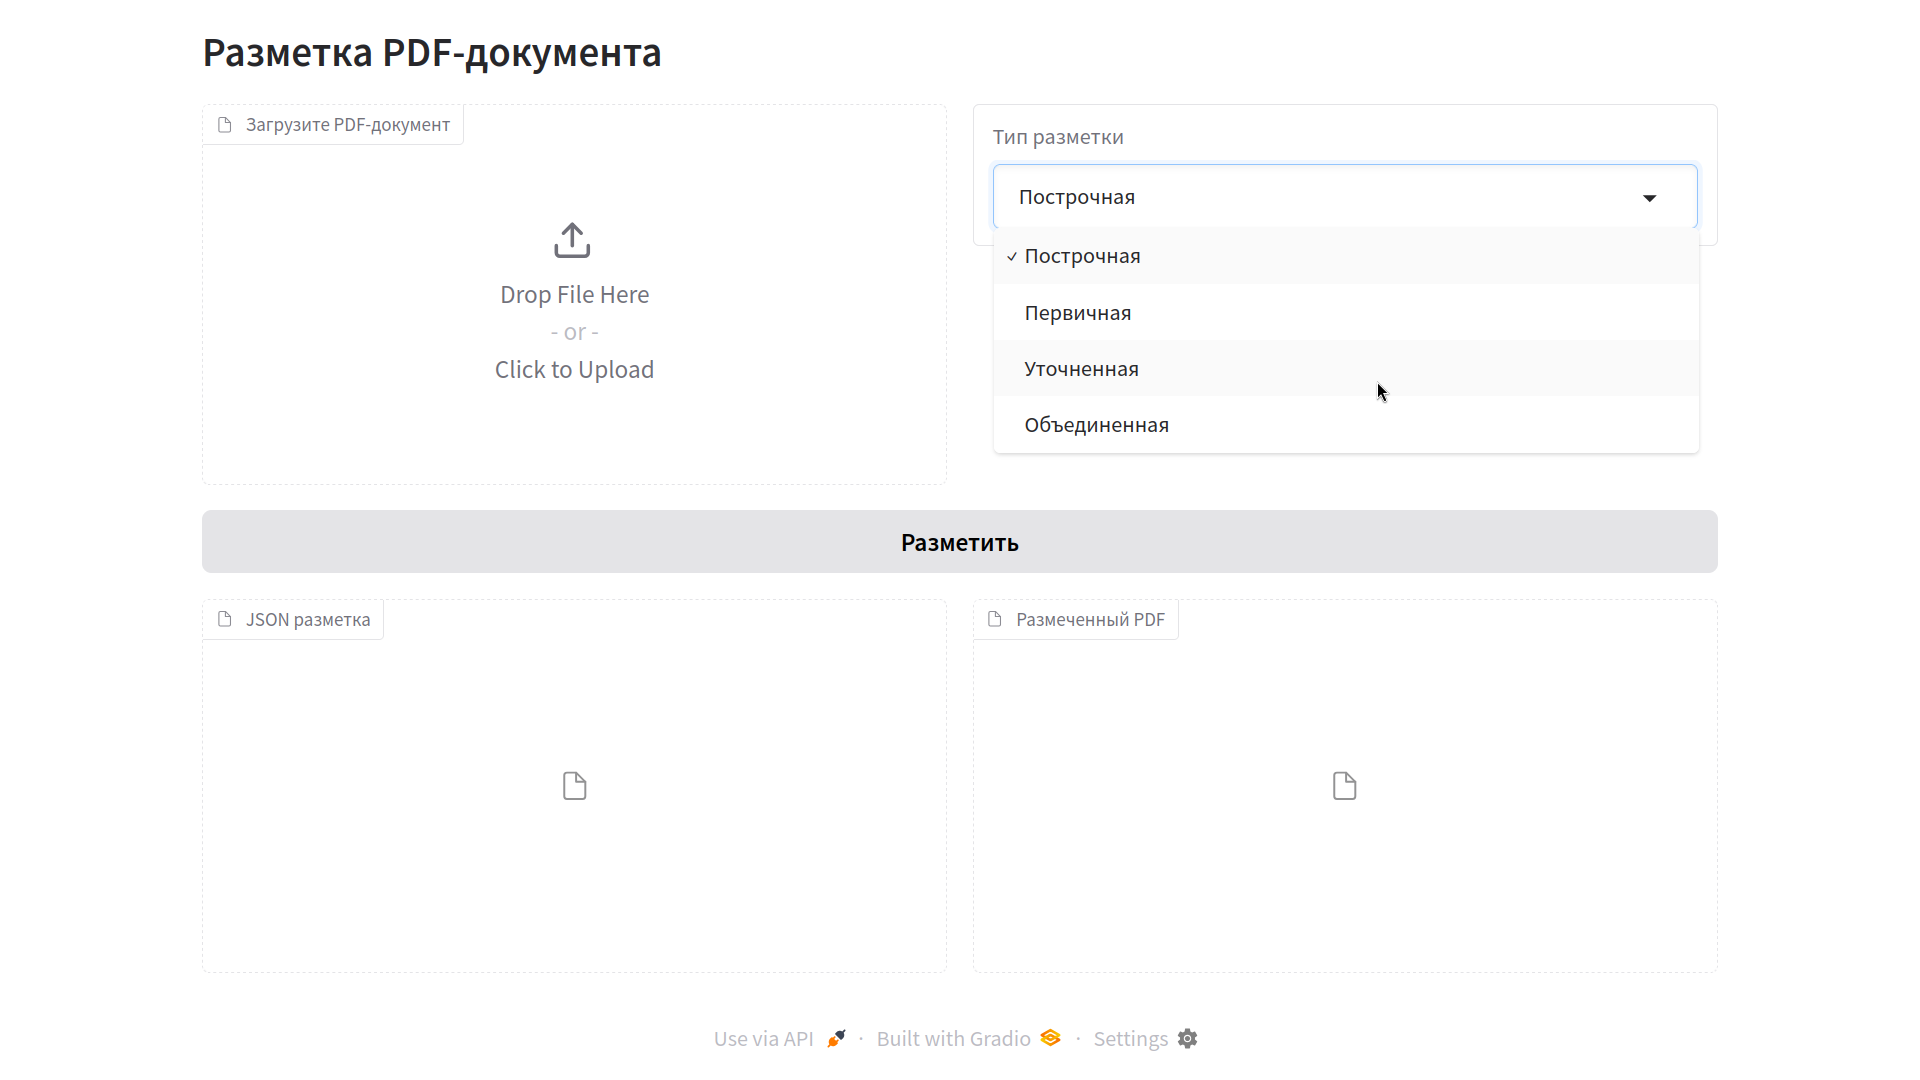
\includegraphics[width=\textwidth]{img/web-start.png}
    \caption{Выбор типа разметки}
	\label{fig:webstart}
\end{figure}

\begin{figure}[H]
	\centering
	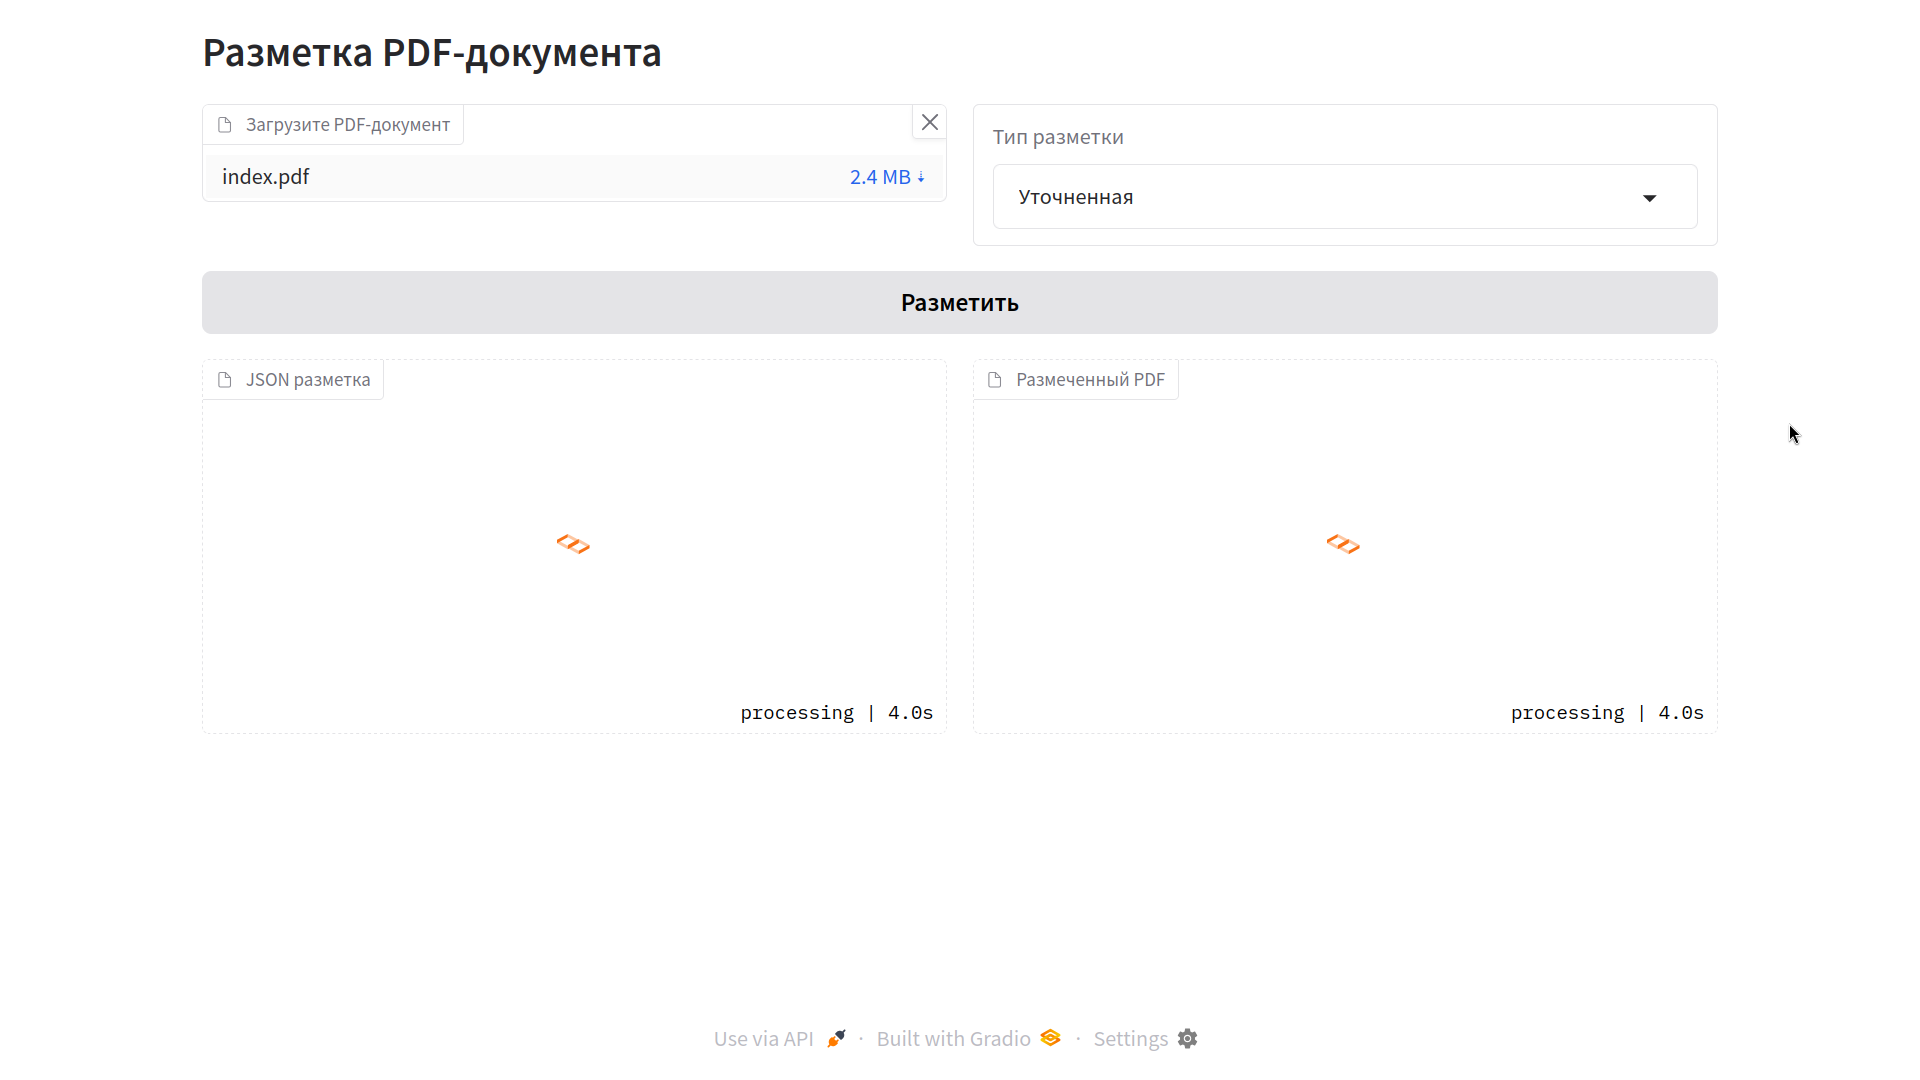
\includegraphics[width=\textwidth]{img/web-process.png}
    \caption{Разметка в процессе}
	\label{fig:webproc}
\end{figure}

\begin{figure}[H]
	\centering
	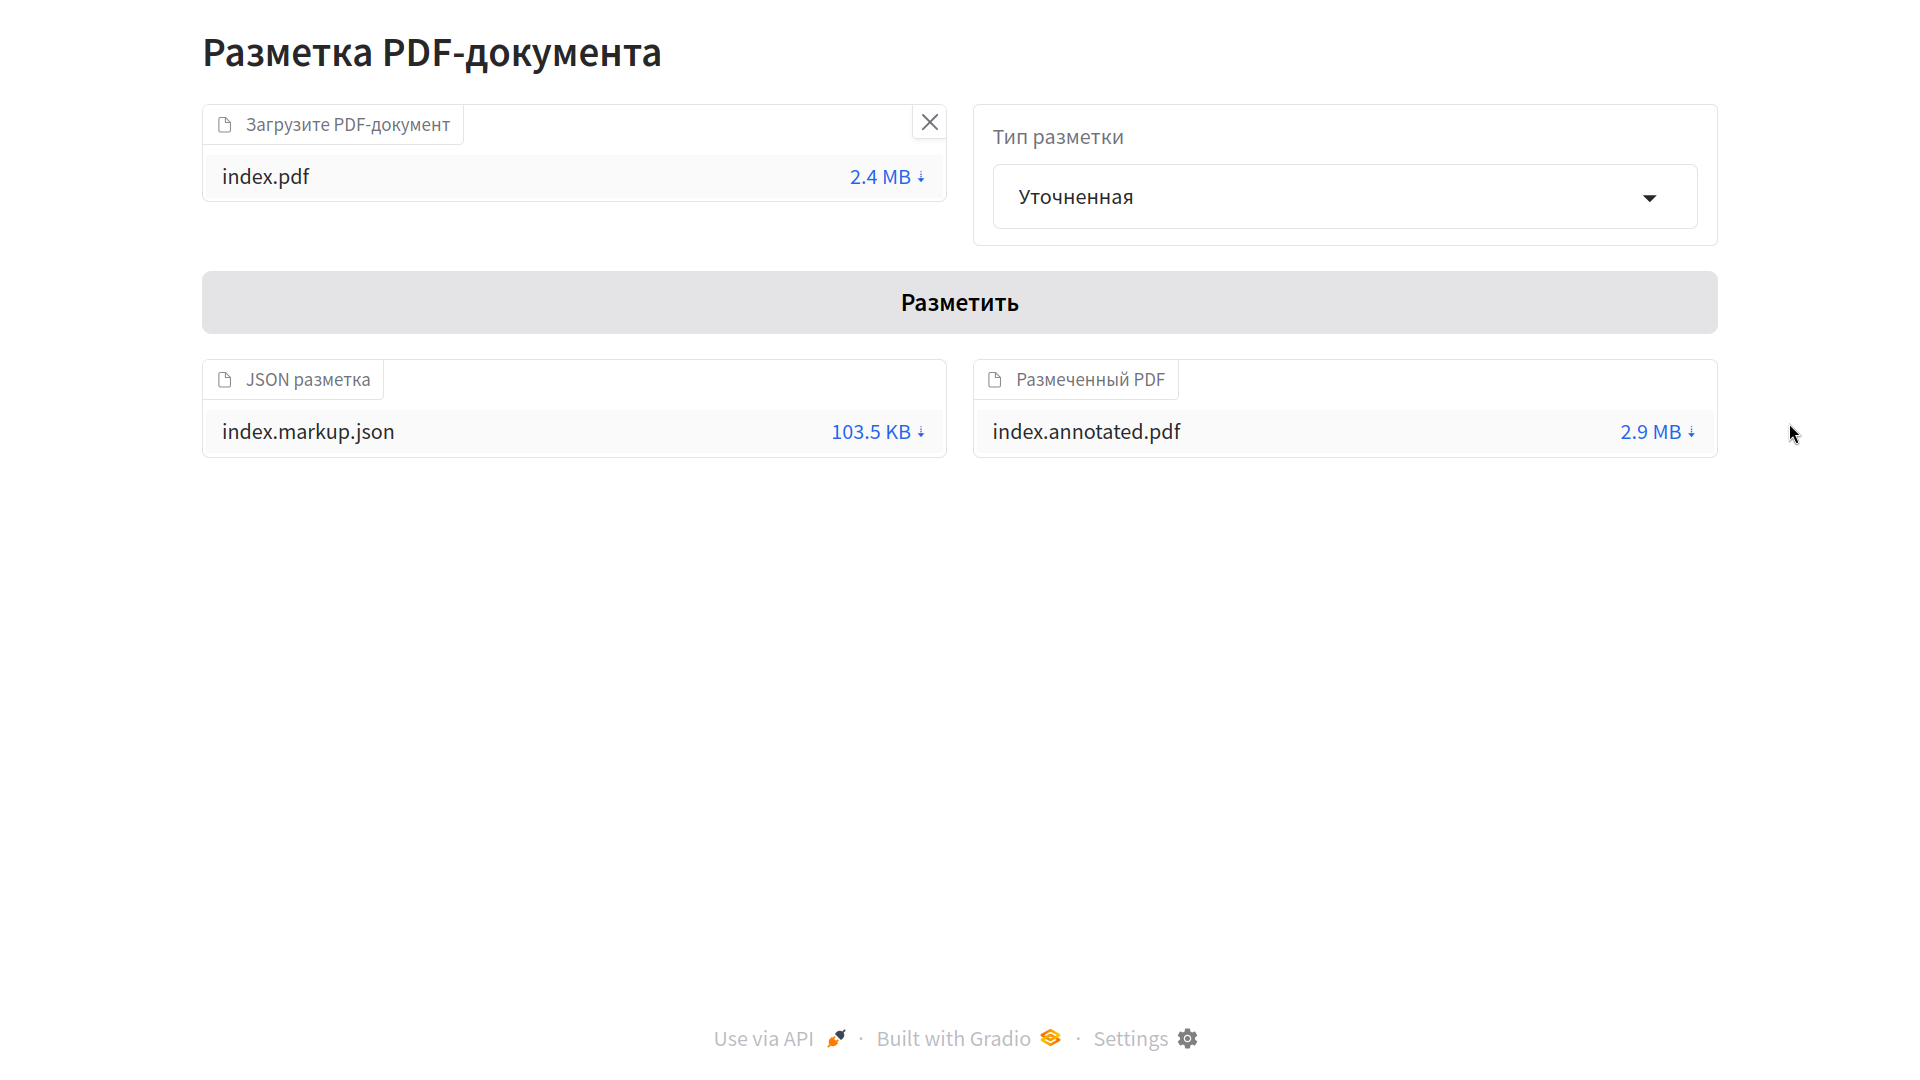
\includegraphics[width=\textwidth]{img/web-done.png}
    \caption{Разметка завершена --- пользователь может скачать разметку в формате JSON и/или PDF документ для ее визуализации}
	\label{fig:webdone}
\end{figure}

\newpage

\subsection{Демонстрация работы программы}

На рисунках \ref{fig:line} -- \ref{fig:merged} ниже приведена демонстрация работы программы.
Представлены результаты построчной (строке пикселей назначется класс на основе распределения пикселей в ней, без использования конечного автомата), первичной, уточненной и объединенной разметок.

\begin{figure}[H]
	\centering
	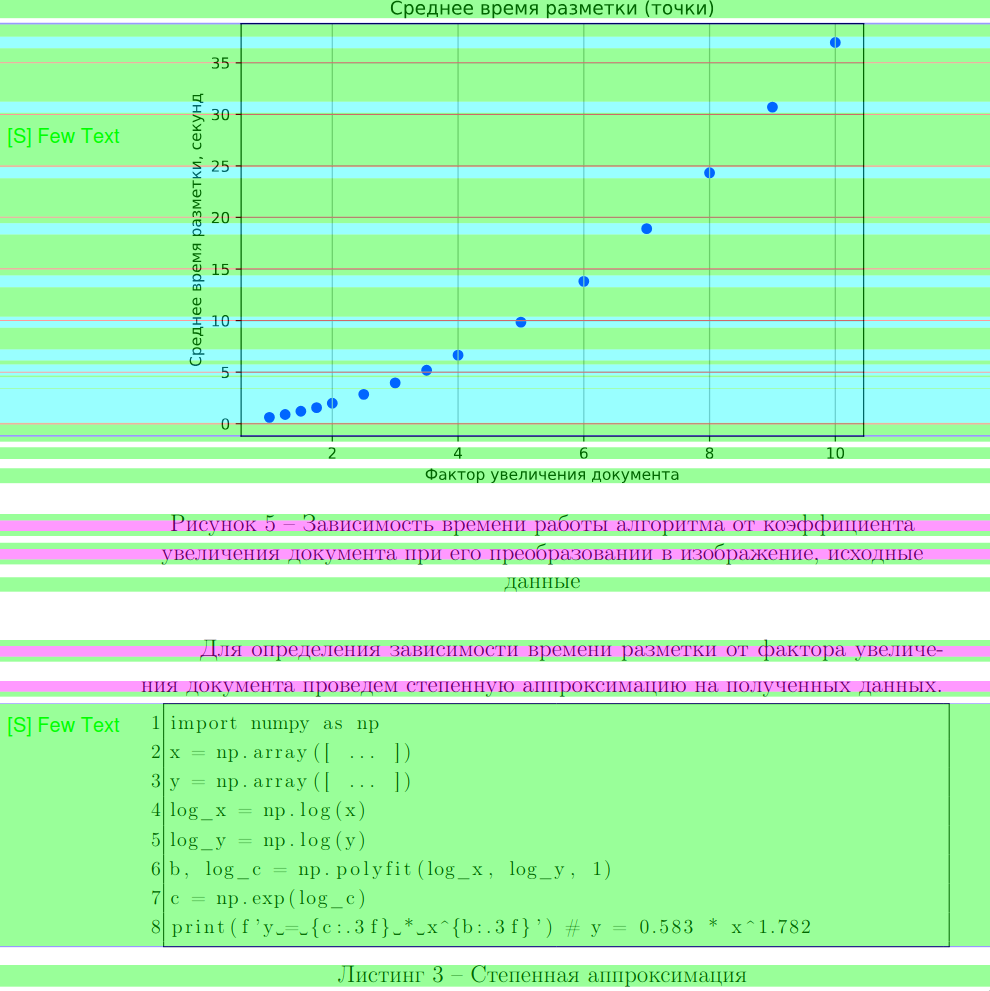
\includegraphics[width=\textwidth]{img/m.line.png}
    \caption{Пример построчной разметки}
	\label{fig:line}
\end{figure}

\begin{figure}[H]
	\centering
	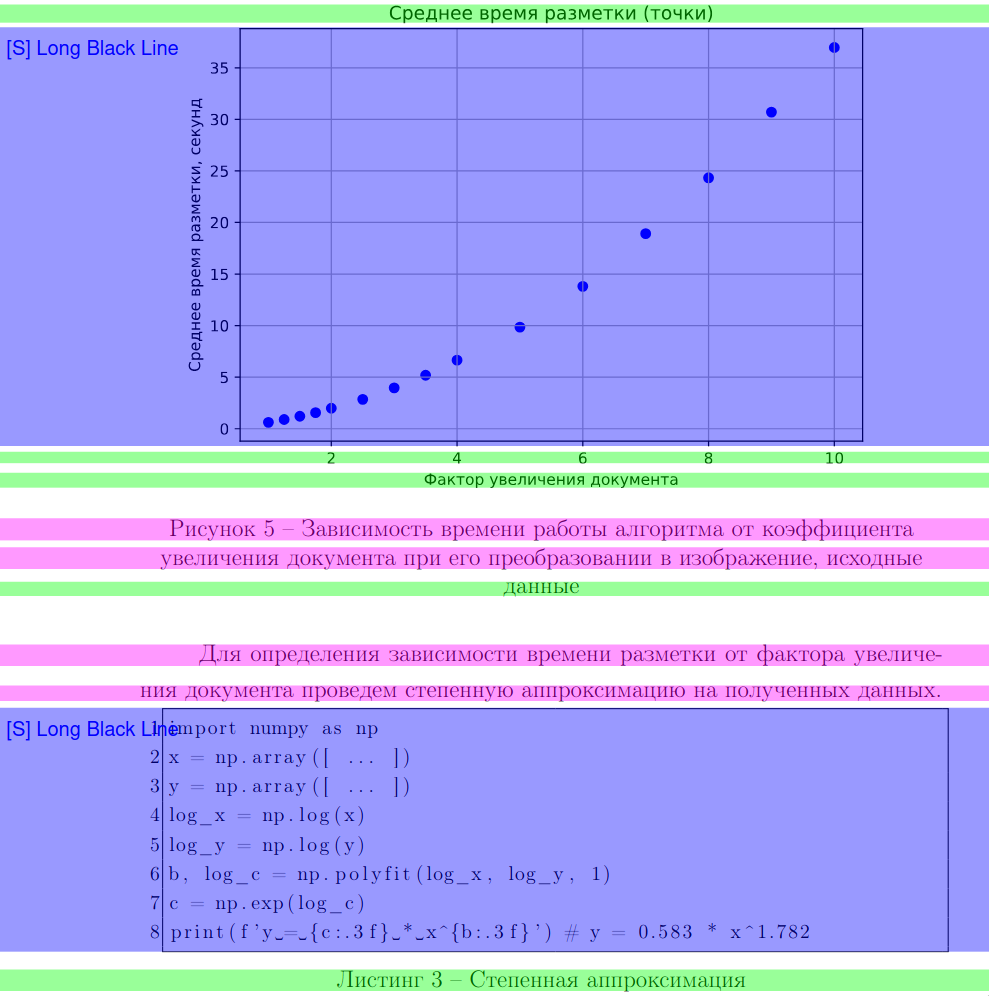
\includegraphics[width=\textwidth]{img/m.prim.png}
    \caption{Пример первичной разметки}
	\label{fig:prim}
\end{figure}

\begin{figure}[H]
	\centering
	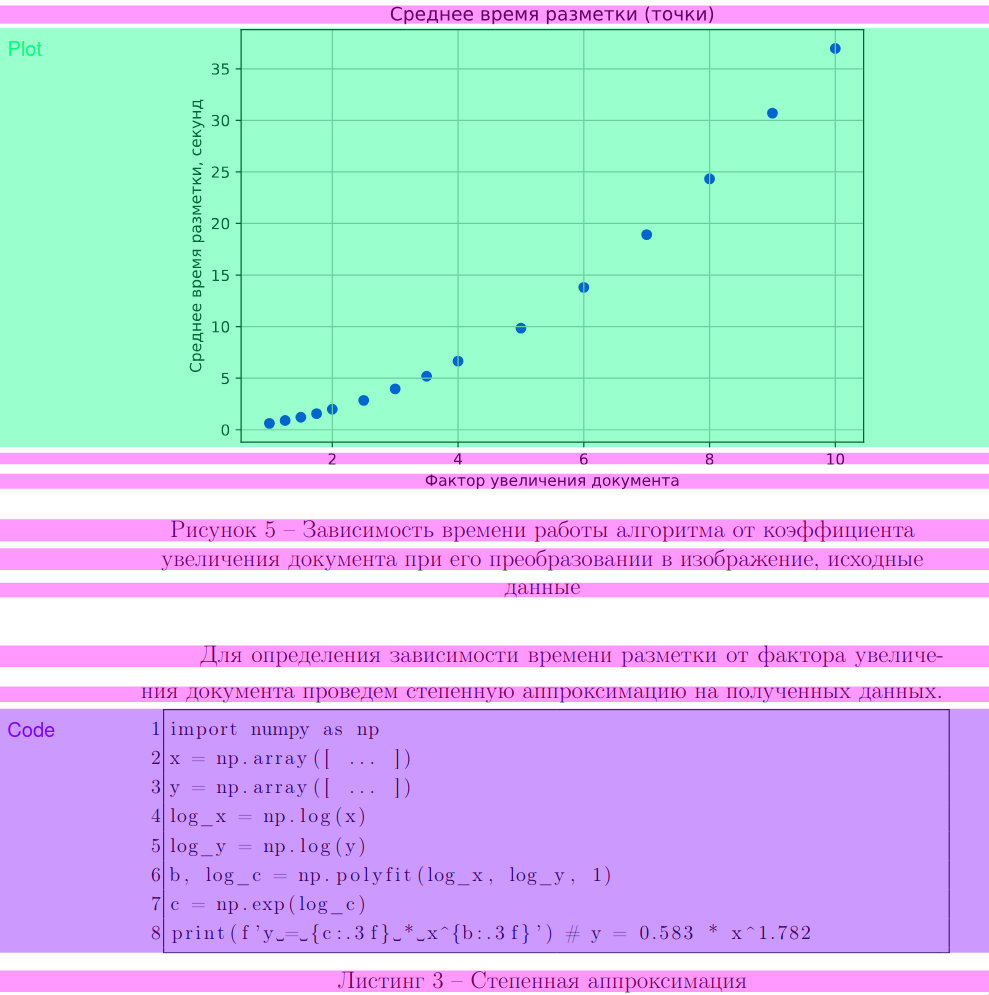
\includegraphics[width=\textwidth]{img/m.spec.png}
    \caption{Пример уточненной разметки}
	\label{fig:spec}
\end{figure}

\begin{figure}[H]
	\centering
	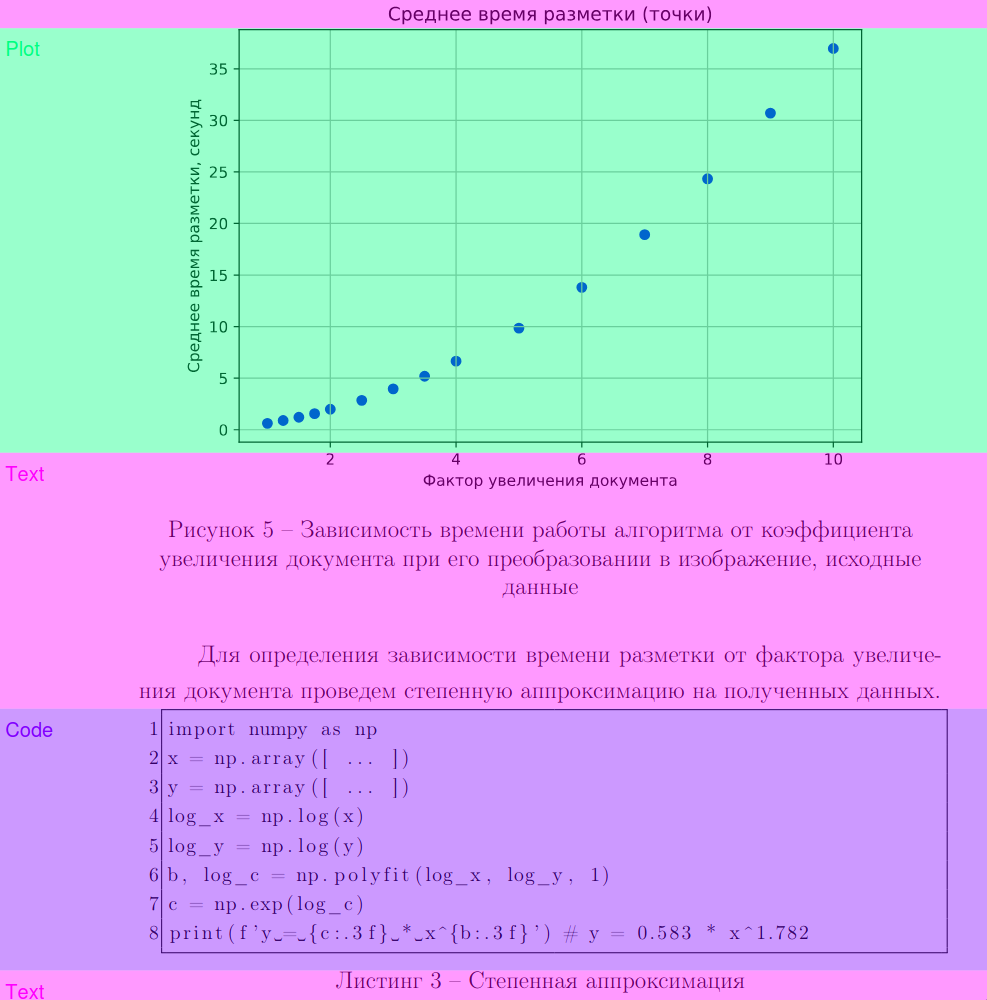
\includegraphics[width=\textwidth]{img/m.merged.png}
    \caption{Пример объединенной разметки}
	\label{fig:merged}
\end{figure}

\newpage

В листингах \ref{lst:main} и \ref{lst:apply} ниже представлен результат работы программы при запуске из терминала.

\begin{lstlisting}[caption={Запуск и результат работы разметки из терминала}, label={lst:main}]
uv run main.py ~/index.pdf x.json 3
Pages processed: 31/31 [00:06<00:00,  5.11it/s]
\end{lstlisting}

\begin{lstlisting}[caption={Запуск и результат применения разметки к PDF из терминала}, label={lst:apply}]
uv run apply.py ~/index.pdf x.json output.pdf
Annotating pages: 31/31 [00:00<00:00, 383.41it/s]
Сохранено в: output.pdf
\end{lstlisting}

\subsection{Руководство пользователя}

Для запуска программы требуется установить uv командой, показанной в листинге~\ref{lst:curl} ниже.
\begin{lstlisting}[caption={Установка uv}, label={lst:curl}]
curl -LsSf https://astral.sh/uv/install.sh | sh
\end{lstlisting}

После установки uv, следует установить зависимости приложения.
Для этого, находясь в директории с программой, следует прописать команду, показанную в листинге~\ref{lst:uvsync} ниже.
\begin{lstlisting}[caption={Установка зависимостей}, label={lst:uvsync}]
uv sync
\end{lstlisting}

Графический интерфейс запускается локально командой, показанной в листинге~\ref{lst:webgui} ниже.
\begin{lstlisting}[caption={Запуск графического веб-интерфейса}, label={lst:webgui}]
uv run webgui.py
\end{lstlisting}

Также можно создать разметку без использования графического интерфейса.
Для этого используется скрипт main.py, инструкция к использованию которого приведена в листинге~\ref{lst:mainpy} ниже.

\newpage

\begin{lstlisting}[caption={Запуск скрипта для создания разметки}, label={lst:mainpy}]
Использование: main.py [-w КОЛИЧЕСТВО_ПРОЦЕССОВ]
                       [-p СТРАНИЦЫ]
                       pdf_path json_path {0,1,2,3}

Сегментировать PDF страницы и экспортировать разметку в JSON.

Позиционные аргументы:
  pdf_path              Путь ко входному PDF файлу
  json_path             Путь к выходному JSON файлу
  {0,1,2,3}             Тип разметки: 0 - построчная разметка,
                                      1 - первичная разметка,
                                      2 - уточненная разметка,
                                      3 - объединенная разметка

Опции:
  -w, --workers КОЛИЧЕСТВО_ПРОЦЕССОВ
                        Количество рабочих процессов
                        (по умолчанию: 8)
  -p, --pages СТРАНИЦЫ  Диапазоны страниц для обработки,
                        например, '1-3,5,7-9'
\end{lstlisting}

Для применения разметки к документу без графического интерфейса используется скрипт apply.py, инструкция к использованию которого приведена в листинге~\ref{lst:applypy} ниже.
\begin{lstlisting}[caption={Запуск скрипта для применения разметки к PDF документу}, label={lst:applypy}]
Использование: apply.py [-h] pdf_path json_path output_path

Разметить PDF цветными сегментами из JSON файла разметки.

Позиционные аргументы:
  pdf_path     Путь ко входному PDF файлу
  json_path    Путь к JSON файлу с разметкой
  output_path  Путь для сохранения размеченного PDF
\end{lstlisting}

\newpage

\subsection*{Вывод}

В данном разделе были выбраны средства реализации программного обеспечения, описаны основные функции разработанного программного обеспечения, приведены результаты тестирования, примеры пользовательского интерфейса, демонстрация работы программы, а также руководство пользователя.
